\chapter{Testing}

This section documents the tests used to ensure that the implementation of Liquid State Machine is functional, and to highlight certain properties of both the implementation and the network model itself, finishing off with a test problem.

\section{Neuron model}

The neuron model is a critical part of this project, and as such should be tested to gain insight of what impacts the firing rate and sensitivity of the model.

In order to test this model, a baseline set of parameters must first be selected. The baseline parameters are as follows; Resistance : 2.2, Time constant : 10, Resting potential : 0, Spiking potential : 1. For these parameters, the model behaves as can be seen in figure \ref{fig:model1} which is clearly a smooth membrane potential curve followed by a spike as the potential reaches the spiking threshold. In figure \ref{fig:model2}, the parameters have been changed to allow a random input between zero and one. This input range is chosen to simulate a set of different synapses providing input to the neuron could behave if the expected sum of their synaptic inputs was in this range, illustrating how a neuron would act when it's input is affected by several synapses that fire independent of each other. It is clear from these two images, as the neuron fires in exactly the same timestep, that the mean input is relevant, even if the input is not consistent.

\begin{figure}
    \centering
    \begin{subfigure}[b]{0.3\textwidth}
        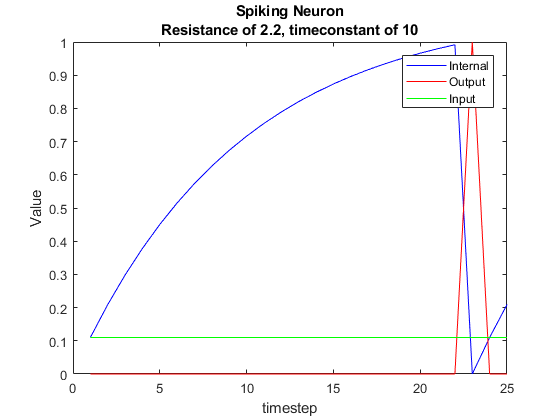
\includegraphics[width=\textwidth]{Images/slow.png}
        \caption{The neuron model using the baseline parameters and constant input of 0.5.}
        \label{fig:model1}
    \end{subfigure}
    \begin{subfigure}[b]{0.3\textwidth}
        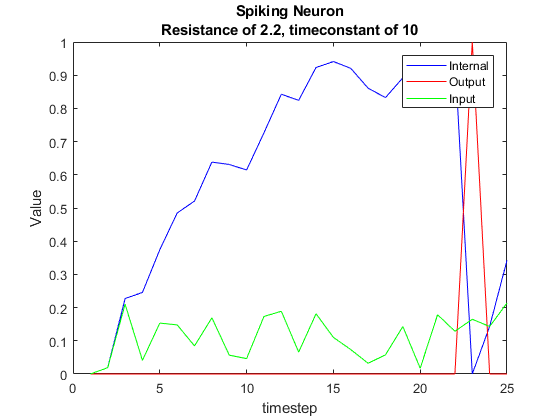
\includegraphics[width=\textwidth]{Images/randomInput.png}
        \caption{The neuron model using the baseline parameters and random input with a mean of 0.5.}
        \label{fig:model2}
    \end{subfigure}
    \begin{subfigure}[b]{0.3\textwidth}
        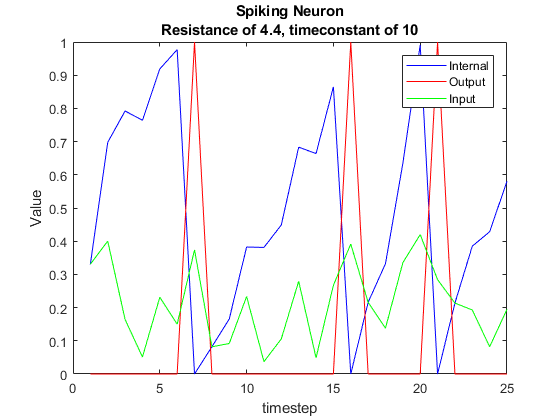
\includegraphics[width=\textwidth]{Images/fast.png}
        \caption{The neuron model using double resistance, and random input with a mean of 0.5.}
        \label{fig:fast}
    \end{subfigure}
    \caption{Tests of the neuron model.(a) shows the ideal potential curve followed by a spike. (b) shows how the potential curve caused by a randomized input can be used in place of the ideal curve to get the same frequency of the spike. (c) shows how resistance parameter is nonproportional to the firing rate.}
    \label{fig:implementation_test}
\end{figure}

If one instead changes the parameters so that the resistance is twice of what it was in the baseline, and sets the input to a random number between zero and one each timestep, the result, as seen in figure \ref{fig:fast}, the neuron fires three times in the same timestep, showing how the resistance is not proportional to the fire rate of the neuron.

\section{Propagation}

In a functional Liquid State Machine, the activation of a neuron in the hidden layer will spread to nearby neurons like ripples in a pond. In order to test this, one can activate a single neuron and observe this behavior through the activation of the connected neurons. One way of performing this observation is by setting the neuron parameters in such a way that a single received pulse is enough to cause an activation, and then activating a single neuron in the reservoir. The expected behavior is a cascade effect where each activation will activate several other neurons, eventually activating each connected neuron in the reservoir.

By visualizing the activity of the network through repeated activations, this is easy to test. In figure \ref{fig:implementation_test}, it is clear that a single reservoir neuron is activated after the first timestep, and that after ten timesteps all connected neurons have been activated. In this figure it is also clear that three adjacent neurons, which is the number of connections each neuron have, are activated in the second timestep, as is expected from a functional Liquid State Machine.

\begin{figure}
    \centering
    \begin{subfigure}[b]{0.225\textwidth}
        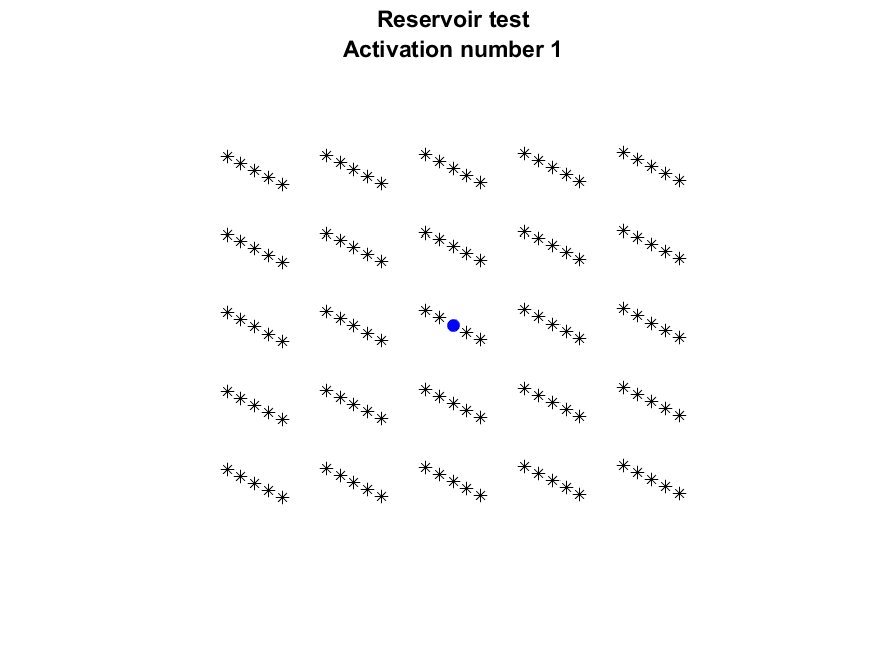
\includegraphics[width=\textwidth]{Images/Reservoir_test_Activation_number_1.png}
        \caption{The test network after a single timestep.}
    \end{subfigure}
    \begin{subfigure}[b]{0.225\textwidth}
        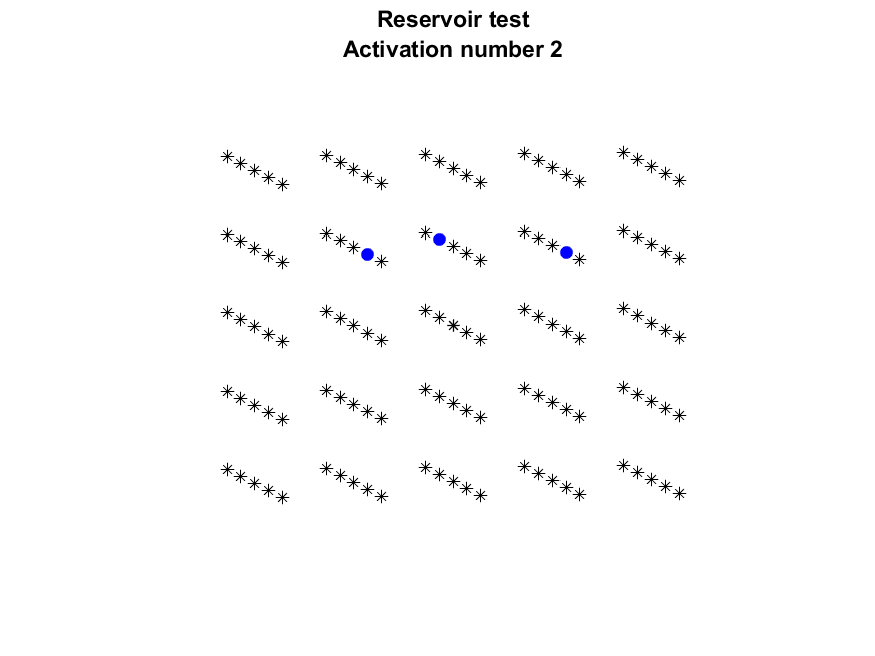
\includegraphics[width=\textwidth]{Images/Reservoir_test_Activation_number_2.png}
        \caption{The test network after two timesteps.}
    \end{subfigure}
    \begin{subfigure}[b]{0.225\textwidth}
        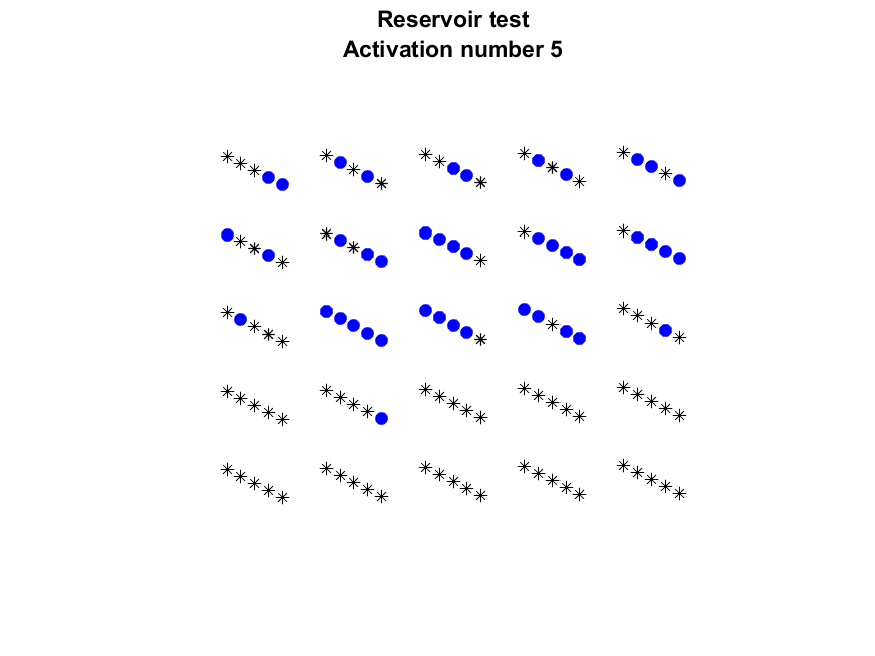
\includegraphics[width=\textwidth]{Images/Reservoir_test_Activation_number_5.png}
        \caption{The test network after five timesteps.}
    \end{subfigure}
     \begin{subfigure}[b]{0.225\textwidth}
        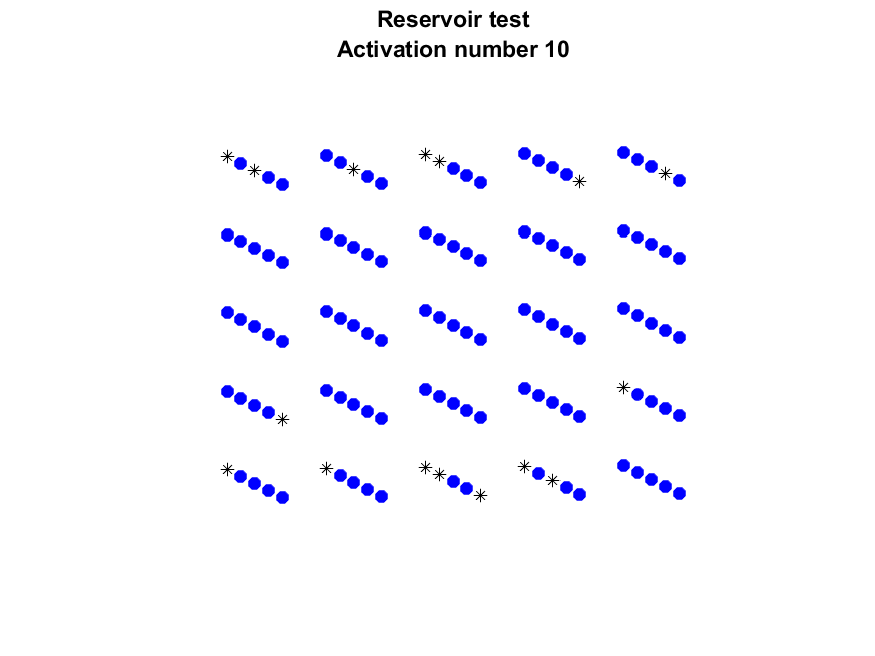
\includegraphics[width=\textwidth]{Images/Reservoir_test_Activation_number_10.png}
        \caption{The test network after ten timesteps.}
    \end{subfigure}
    \caption{Test of the propagation of the network. Every neuron has three synapses which are adjacent to it, and each spike will activate all three synases. After the first timestep, only the selected neuron is active. In the second timetep, it has spiked and is therefore inactive while the three neurons it has synapses to are active. After five timesteps a large proportion of the neurons are active, and after ten all connected neurons are active.}
    \label{fig:implementation_test}
\end{figure}

\section{Reservoir activity}

The reservoir parameters are as important as the neuron parameters. There are several parameters that can be tuned and modified, and in this section the number of connections as well as the proportion of exitory to inhibitory neurons are tuned. The rest of the parameters are kept constant, as well as the neuron parameters, which are as follows; Resistance : 2.2, Time constant : 10, Resting potential : 0, Spiking potential : 1, Minimum weight : 0, Maximum weight : 1, Max synapse length : 2, Number of input neurons : 3, Number of connections per input neuron : 10.

 Having too few connections will result in low amount of activity that won't spread beyond the input neurons. Conversely, having too many connections will result in a cascade of activity that results in all, or most, neurons activating every timestep. Both of these options are equally useless, as they provide essentially constant output.

First, to test the impact of the number of connections that each neuron have on the level of activity of the reservoir, two different amounts of neuron connections are tested. The reservoir after one hundred timestept with six and seven connections per neuron can be seen in figure \ref{fig:reservoir_6} and \ref{fig:reservoir_7}. As can be seen in the first image, six connections are enough to provide a good level of activity throughout the network, without having a lot of the neurons activate each timestep. On the other hand, having seven connections is enough to cause a run-away reaction that activates almost all the neurons each timestep. Clearly, there is a fine balance between having enough connections, and having too many.

A way of correcting this is by including inhibitory neurons. In figure \ref{fig:reservoir_7_in} we see how 15\% inhibitory neurons brought the level of activity back down, and in figure \ref{fig:reservoir_10_in}.

\begin{figure}
    \centering
    \begin{subfigure}[b]{0.225\textwidth}
        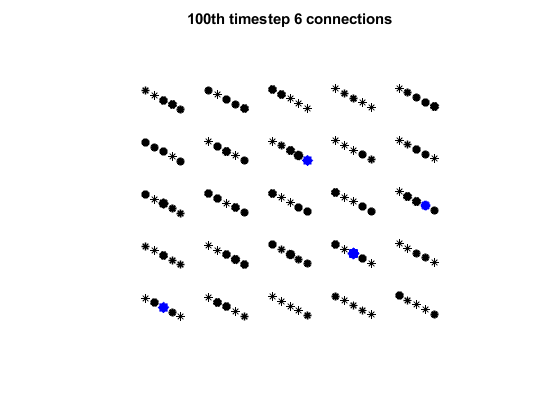
\includegraphics[width=\textwidth]{Images/pool_6_100.png}
        \caption{The test network after a hundred timesteps with 6 connections per neuron.}
    \label{fig:reservoir_6}
    \end{subfigure}
    \begin{subfigure}[b]{0.225\textwidth}
        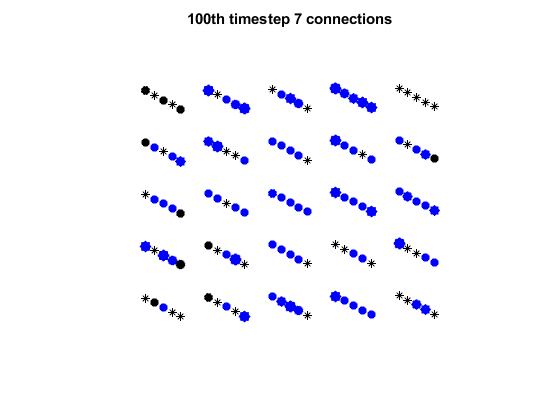
\includegraphics[width=\textwidth]{Images/pool_7_100.png}
        \caption{The test network after a hundred timesteps with 7 connections per neuron.}
    \label{fig:reservoir_7}
    \end{subfigure}
    \begin{subfigure}[b]{0.225\textwidth}
        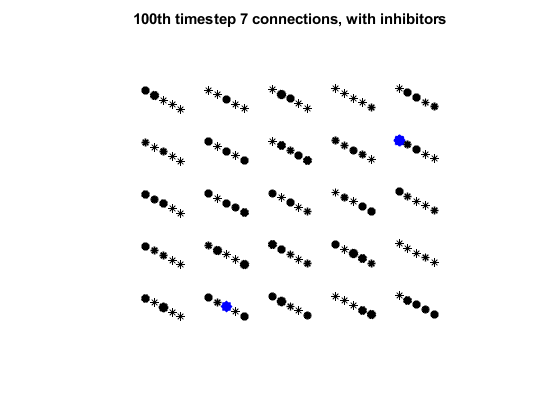
\includegraphics[width=\textwidth]{Images/pool_7_100_s.png}
        \caption{The test network after a hundred timesteps with 7 connections per neuron, with inhibitors.}
    \label{fig:reservoir_7_in}
    \end{subfigure}
     \begin{subfigure}[b]{0.225\textwidth}
        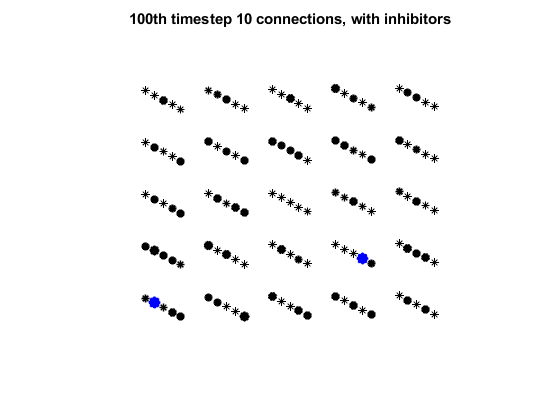
\includegraphics[width=\textwidth]{Images/pool_10_100_s.png}
        \caption{The test network after a hundred timesteps with 10 connections per neuron, with inhibitors.}
    \label{fig:reservoir_10_in}
    \end{subfigure}
    \caption{Spikes and membrane potential after a hundred timesteps with different amounts of connections per neuron and inhibitors.}
\end{figure}

\section{Sequence prediction}

In order to test the full implementation, a test problem was chosen. This test problem is a classification problem on a continous sequence of "AAABBBCCC", using the Liquid State Machine to predict the next input in the sequence.

In order to train the network to this sequence, every input is continued for ten timesteps, equal to the time constant. The parameters for the neurons and reservoir are; Resistance : 3.3, Time constant : 10, Resting potential : -0.1, Spiking potential : 1, Minimum weight : 0.5, Maximum weight : 1, Max synapse length : 1, Number of input neurons : 3, Number of connections per input neuron : 100, Learning rate : 0.0001, Proportion of inhibitory neurons : 25\%.

The training and testing is carried out by first creating the input for 1.200.000 timesteps. The first 90\% is used for training, and the remainding 10\% for testing.

In image \ref{fig:result} the outputs for the last 300 timesteps are shown, and in image \ref{fig:resultMean} the outputs for the ten timesteps per sequence element is meaned. It is clear from the first image that the signal is somewhat unstable, which is supported by the accuracy of the network when looking at individual timesteps, which is 82\%. The second image, in contrast, is much more stable, and indeed has an accuracy of 100\% for the entire test set.

\begin{figure}
    \centering
    \begin{subfigure}[b]{0.4\textwidth}
        \includegraphics[width=\textwidth]{Images/LSM.png}
        \caption{The last 300 timesteps for the test data.}
    \label{fig:result}
    \end{subfigure}
    \begin{subfigure}[b]{0.4\textwidth}
        \includegraphics[width=\textwidth]{Images/LSMmean.png}
        \caption{The last 300 timesteps for the test data, meaned outputs.}
    \label{fig:resultMean}
    \end{subfigure}
    \caption{Outputs for the sequence prediction test.}
\end{figure}










